\chapter{超导量子比特的基本原理}
\section{超导量子计算的历史}
半导体技术的快速发展深刻改变了人类生活的各个方面,引领人类进入信息时代。计算能力也由此成为基础设施的核心组成部分,成为衡量国家综合国力的标准之一。但当前半导体工艺的发展已经受到量子力学的限制,计算能力的提升也逐渐陷入瓶颈。如何进一步提高计算能力成为萦绕在人们心头的重要问题。量子计算作为一种遵循量子力学规律进行计算的新型计算模式,在某些特定问题上展现了远超经典计算机的计算能力,引起了学术界和工业界的极大关注\cite{braumuller2022probing,arute2019quantum,jurcevic2021demonstration}。

2000年,DiVincenzo提出了五条准则,只有满足这五条准则的物理体系,才能构建出可行的量子计算机。这五条准则分别为\cite{divincenzo2000physical}:
\begin{enumerate}
	\item 可拓展量子系统中具有可表征的量子比特;
	\item 系统可以将状态初始化到一个基准态,例如$\ket{000\cdots0}$;
	\item 系统的退相干时间远大于量子门操作的时间;
	\item 具有一套通用的量子门操作;
	\item 具有量子比特的特定量子态读取能力;
\end{enumerate}

满足这些准则的物理体系有许多种,包括超导电路\cite{havlivcek2019supervised,google2020hartree},离子阱\cite{erhard2019characterizing,zhang2017observation},光子\cite{zhong2020quantum,zhong2021phase},中性原子\cite{semeghini2021probing,bernien2017probing}等体系。其中超导电路体系以其高拓展性,易操控性,以及对当前先进半导体工艺的高兼容性,成为了目前主流的量子计算机实现体系之一,获得科学界和工业界的高度关注\cite{braumuller2022probing,arute2019quantum,jurcevic2021demonstration}。总体来说,超导量子计算有以下几个优点:
\begin{enumerate}
	\item 具有很高的设计自由度:可以设计成不同的电路结构以及不同的电路参数。
	\item 可拓展性:当前超导量子处理器的制备工艺和当前先进半导体工艺是高度兼容的,有利于其制备和拓展。
	\item 易耦合性:通过设计电容和电感等电路参数,可以简单地构成比特间的耦合。
	\item 易操控性:超导量子比特的控制主要通过微波信号和射频信号,已经有成熟的商业设备对其进行支持。
\end{enumerate}

1985年,John Clark首次观察到偏置电流约瑟夫森结的量子行为\cite{devoret1985measurements}。随后,在1998年,Michel Devoret证明了电荷量子比特的叠加态的存在\cite{bouchiat1998quantum}。1999年日本研究小组 Nakamura等人设计并制造出了第一个超导量子比特,实现了对宏观量子态的相干控制\cite{nakamura1999coherent}。最初的超导量子比特仅有几纳秒的相干时间,这无法满足计算过程的需求\cite{nakamura1999coherent}。

为了提高量子比特的性能和相干时间,研究人员探索了各种不同类型的量子比特,如电荷量子比特\cite{vion2002manipulating}、磁通量子比特\cite{chiorescu2003coherent}、相位量子比特\cite{simmonds2004decoherence}等。2007年,Devoret研究小组设计出传输子量子比特(transmon)\cite{koch2007charge},这种新型结构的比特结合了多种不同设计方案的优点,拥有相干性好、复杂度低、便于操控与读取等优点,逐渐成为最主流的超导比特方案。近些年来,传输子量子比特的退相干性能,操控性能,以及集成性能都得到了显著的提升\cite{arute2019quantum,wu2021strong}。经过微纳加工制备工艺和薄膜材料的改进,单独的传输子量子比特的能量弛豫时间最高能达到$500\ {\mu s}$\cite{place2021new,wang2021transmon}。在多比特系统中,平均的能量弛豫时间也能达到几十微秒\cite{zhu2022quantum,krinner2021realizing,guo2021stark},甚至百微秒\cite{jurcevic2021demonstration},这些都大大降低了量子计算过程中的非相干错误。超导量子比特的单比特门操作,双比特比特操作和状态读取的保真度也都已经超过了$99\%$\cite{li2019realisation,walter2017rapid,sunada2022fast},超过了量子纠错的错误率阈值,并以此对表面码进行了一系列实验探索。此外,超导量子计算处理器的集成度也大幅度增加,从一维链的九比特结构\cite{kelly2015state},十二比特结构\cite{yan2019strongly,zha2020ergodic},发展到准二维的二十四比特结构\cite{chen2021observation},到二维网格状的六十六比特结构\cite{wu2021strong,zhu2022quantum},一百二十七比特。最新的研究结果显示,超导量子计算处理器的集成度已经高达四百三十三比特\cite{IBMQuantum2022},处理器集成度的发展呈现出加速态势。为了在处理器上集成更多的量子比特,在未来还可能会将倒装焊工艺和深硅通孔工艺相结合,对量子处理器进行3D封装\cite{mallek2021fabrication,rosenberg20193d,vahidpour2017superconducting},以便于信号线的引出,这也是未来超导量子处理器可能的发展方向。

随着超导传输子量子比特的退相干性能,操控性能,和集成性的快速发展,超导量子计算机的计算能力也在大幅度提升。2019年,谷歌量子计算团队在一个五十四比特超导量子计算处理器上进行20层深度的随机线路采样实验\cite{arute2019quantum},该实验的一次采样流程需要花费$200\ {s}$的时间,而同样的问题在最先进的经典超级计算机Summit上进行计算,需要花费大约10000年的时间。此实验结果首次证明了量子计算机在某些特定问题上,具有远超经典计算机的计算能力。虽然在随后几年,随机线路采样问题的经典算法得到不断优化,经典计算机的计算时间已经与谷歌五十四比特量子处理器的时间相当\cite{guo2021verifying}。但是在2021年,中科大潘建伟团队成功在六十六比特量子处理器上进行了同样的24层深度的随机线路采样实验,其时间复杂度比谷歌团队的实验高出六个数量级。在量子处理器上进行的采样实验需要花费4.2小时,而在经典超级计算机上使用最新的经典随机线路采样算法进行同样的采样实验,需要花费4.8万年\cite{zhu2022quantum}。这一结果重新验证了了量子计算的优越性。

超导量子计算机在过去的二十多年里历经了快速的发展,已经从单个量子比特的构建、操控,发展到了四百三十三个高性能量子比特及其高精度操控,并且证明了量子计算相对于经典计算潜在的优越性能。虽然目前距离实用化的可容错通用量子计算机还有不小的距离,但是超导量子计算机的高速发展和巨大的潜在应用能力都吸引着科研人员前仆后继地踏上量子计算研究之路。
\section{超导量子计算系统的结构}
超导量子计算系统的结构如下图\ref{fig:architecture}所示,有两个组成部分,第一部分是系统的核心部分——超导量子处理器,其用于量子信息的处理,整个量子计算过程都在超导量子处理器上进行;另一部分是经典的测量与控制系统,这部分是量子处理器的支撑系统,用于维护量子处理器的量子状态,以及测量与控制信号的生成与传输。

\begin{figure}[h]
	\centering
	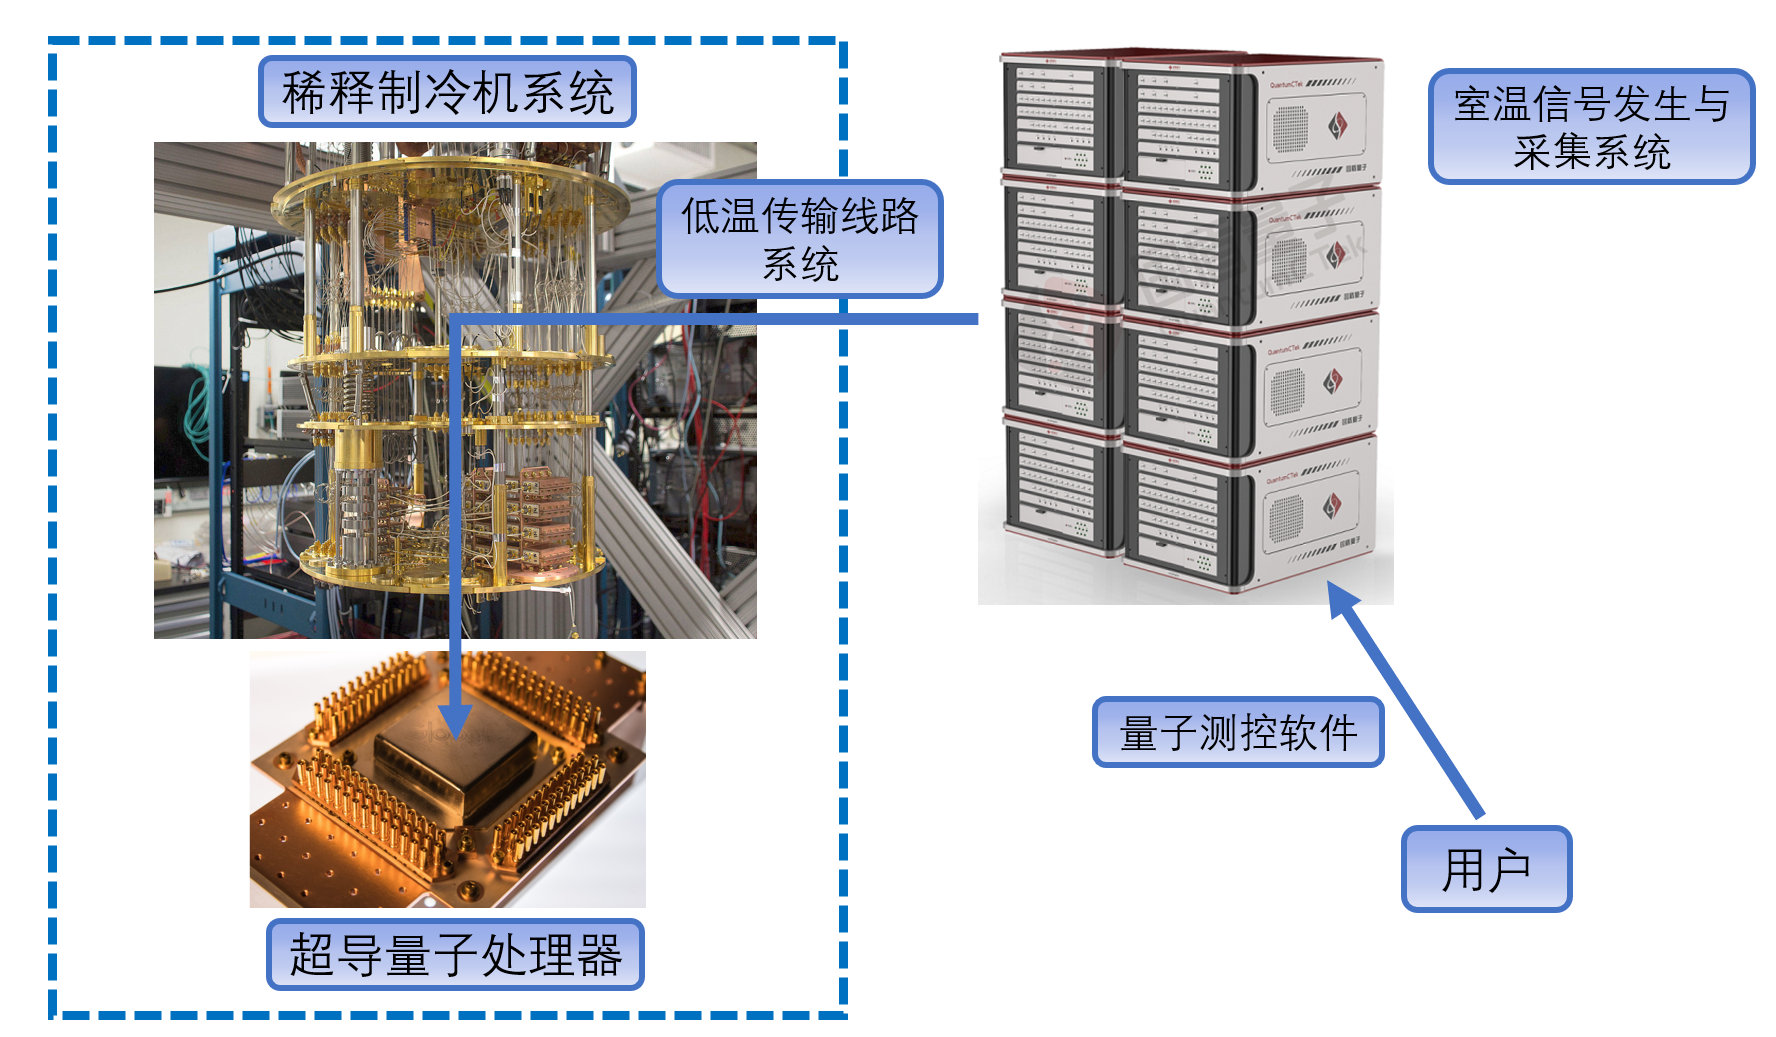
\includegraphics[width=0.9\textwidth]{architecture.png}
	\caption{超导量子计算系统的结构}
	\label{fig:architecture}
\end{figure}

对于用户,会从上位机提交想要运行的量子线路,量子测控软件将量子线路编译成测量与控制系统中经典硬件部分可以理解的语言,将其传输给测控系统。测控系统生成并传输相应微波信号给超导量子处理器,处理器上的量子比特进行相应的量子状态变化,完成用户提交的量子线路对应的量子演化过程,获得最终的量子计算结果。

接下来,我们分别介绍超导量子计算系统的超导量子处理器部分和测量与控制系统部分。
\section{超导量子处理器}
比特是经典计算和经典信息论中的基本概念,是构成经典计算机的基本单元。量子比特是比特在量子计算和量子信息论中的对应,是量子处理器的基本单元。只有构建一个高性能的量子比特,才能在此基础之上进行状态的初始化,操纵和读取,从而进行量子计算过程,这是量子计算的根源。在超导量子计算中,超导量子比特是超导量子处理器的基本单元,是由超导约瑟夫森结构成的谐振电路,因此我们将从LC谐振电路的量子化出发,通过引入超导量子比特的核心器件——约瑟夫森结,介绍超导量子比特的基本原理。
\subsection{LC谐振电路的量子化}
首先介绍LC谐振电路,一个LC谐振电路是由一个线性电感$ L_{c}$和一个线性电容$ C_{c}$并联构成,如下图\ref{fig:EL}a所示。根据电路的基尔霍夫定律:
\begin{equation}
	\begin{split}
		\frac{Q}{C_{c}}-\frac{{d}\Phi}{{d}t}=0, & \\
		\frac{{d}Q}{{d}t}+\frac{\Phi}{L_{c}}=0, & 
	\end{split}
\end{equation}
其中$ Q$为电容极板上所带电荷量,$ \Phi$为电感的磁通量。将两个方程联立,得到$ C_{c}\frac{{d}^{2} \Phi}{{d}t^{2}}+\frac{\Phi}{L_{c}}=0$。这个方程类似于一维谐振子的运动方程,其中$\Phi$等价于运动方程中的坐标$\ x$。根据这个运动方程,我们可以推导出系统的哈密顿量为:
\begin{equation}\label{LCHamilton}
	H = P\times\dot{\Phi}-L = \dfrac{Q^{2}}{2C_{c}}+\dfrac{\Phi^{2}}{2L_{c}},
\end{equation}
\begin{figure}[h]
	\centering
	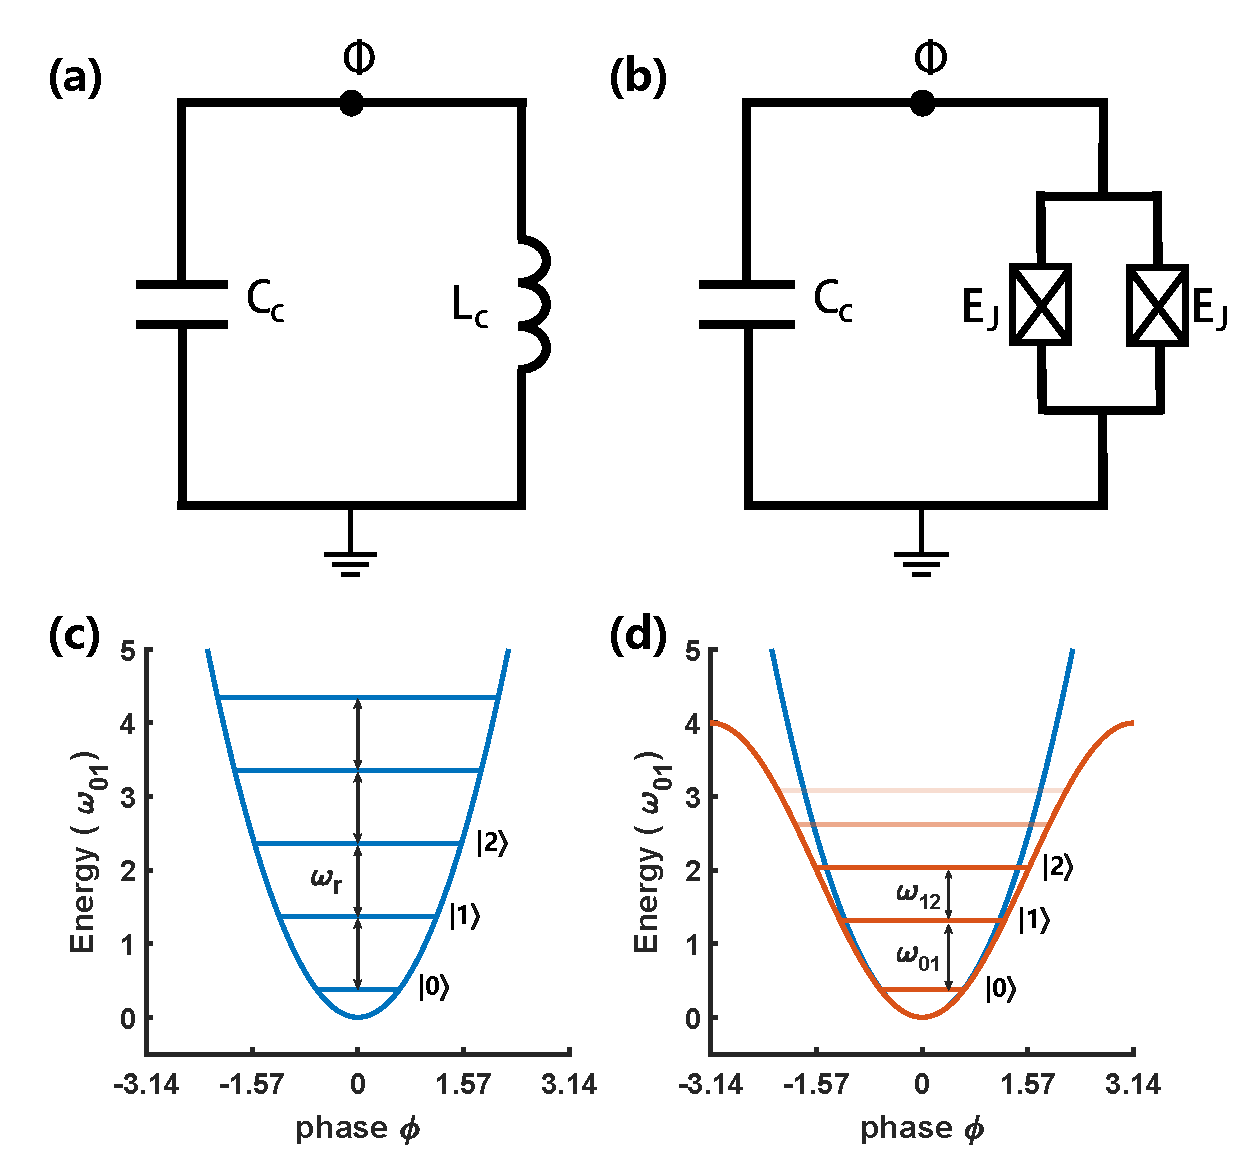
\includegraphics[width=0.9\textwidth]{EL.pdf}
	\caption{谐振电路与传输子量子比特的电路结构和能级结构。(a)谐振电路的集总电路结构示意图。谐振电路由线性电容和电感组成的。(b)传输子量子比特的集总电路示意图。传输子量子比特由线性电容和非线性的约瑟夫森结组成。(c)谐振子系统的能级结构示意图。各个能级之间是等间距的。(d)传输子量子比特的能级结构。其能级之间是不等间距的,$\ket{0}$能级和$\ket{1}$能级与其他能级分隔开,构成了计算空间。}
	\label{fig:EL}
\end{figure}
这是一个明显的谐振子哈密顿量,对其进行二次量子化。令
\begin{equation}
	\begin{split}
		\Phi &= \frac{\sqrt{2\hbar}}{2}(\frac{L_{c}}{C_{c}})^{1/4}\left(\hat{a}+\hat{a}^{\dagger}\right),\\
		Q &= \frac{-\sqrt{2\hbar}{i}}{2}(\frac{C_{c}}{L_{c}})^{1/4}\left(\hat{a}-\hat{a}^{\dagger}\right),
	\end{split}
\end{equation}
并将其带入\ref{LCHamilton}式中,得到LC谐振电路的二次量子化哈密顿量为$ H = {\hbar}\omega\left( \hat{a}^{\dagger}\hat{a}+\frac{1}{2}\right) $,其中$ \omega=2\pi/\sqrt{L_{c}C_{c}}$,是LC谐振电路的谐振角频率,LC谐振电路能级结构如下图\ref{fig:EL}c所示。

LC谐振电路的能级结构是等间隔的,将系统从$\ket{0}$能级驱动到$\ket{1}$能级和将系统从$\ket{1}$能级驱动到$\ket{2}$能级,所需要的微波频率是一致的。这就导致当用微波驱动LC谐振电路系统时,能量不是在$\ket{0}$和$\ket{1}$能级间振荡,而是系统的$\ket{2}$能级,甚至更高能级都会被激发,最终整个系统形成一个相干态,这并不是量子计算过程所需要的结果。我们希望的是将$\ket{0}$,$\ket{1}$能级与其余能级分隔开,构成一个二能级系统,用$\ket{0}$态和$\ket{1}$态编码0和1。在这个二能级系统中,所有的操作都局限在$\ket{0}$,$\ket{1}$展开的计算子空间内,这就需要在哈密顿量中引入非线性的项,以此在量子比特中引入非简谐性。

\subsection{超导约瑟夫森结}
我们通过在LC谐振电路中添加超导约瑟夫森结来引入非线性项。超导约瑟夫森结是由两个超导体和中间的一个薄的非超导体组成的,如下图\ref{fig:Josephson}所示,是约瑟夫森在1962年首次在理论上预言\cite{josephson1962possible},并于1963年被P.W.Andetson和J.M.Rowell在实验上证实\cite{anderson1963probable}。

当导体进入超导态后,费米面附近的电子相互吸引,形成了大量的库伯对。这些库伯对彼此交叠渗透,保持相同的有序度,构成一个电子的整体行为。我们可以利用波函数$ \Psi(r)=\sqrt{\rho(r)}{e}^{{i}\varphi(r)}$来描述这些电子的集体行为,其中$ \sqrt{\rho}$是波函数的振幅,$ \varphi$是其相位。每个相互独立的超导体都有各自独立的波函数来描述。当两个超导体通过一个薄的非超导体相连接,构成约瑟夫森结,两个超导体之间发生弱了耦合,两个波函数之间就不再相互独立,而是存在一定的线性关系。
\begin{figure}[h]
	\centering
	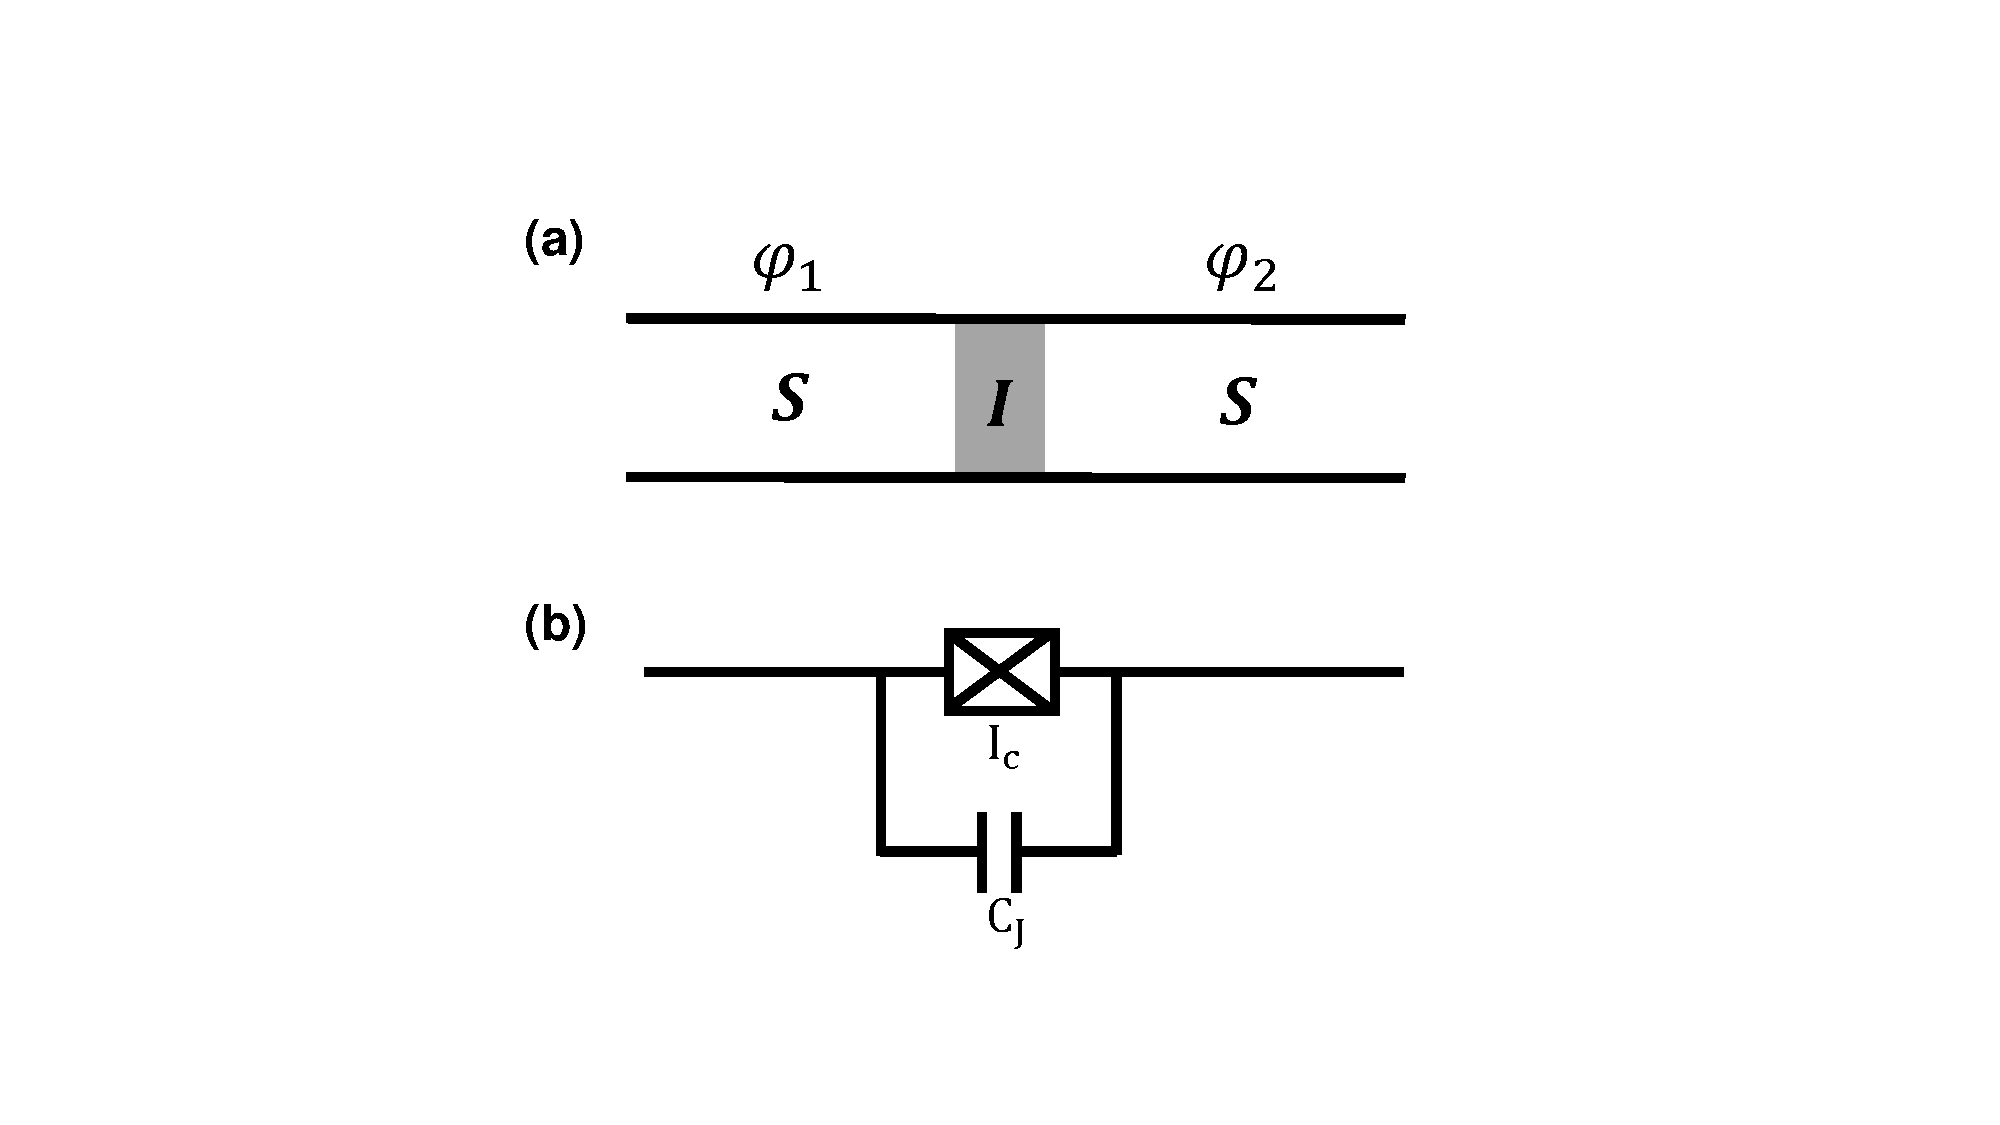
\includegraphics[width=0.6\textwidth]{Josephson.pdf}
	\caption{超导约瑟夫森结结构。(a)超导约瑟夫森结的物理结构。S代表超导体,I代表绝缘层,$ \varphi_{1}$、$ \varphi_{2}$分别是两个超导体内部电子的相位。(b)超导约瑟夫森结的实际电路结构,一般由完美的约瑟夫森结并联一个结电容组成,约瑟夫森结的特征电流为$ I_{c}$,一般结电容$ C_{J}= 9\ {fF}$。}
	\label{fig:Josephson}
\end{figure}

根据这个线性关系,再利用薛定谔方程和微扰论的方法,我们可以求得约瑟夫森结所遵循的约瑟夫森方程,该方程描述的是约瑟夫森结两端的电压$ V$,隧穿电流$ I$和约瑟夫森结两端超导体的相位差$\varphi$之间的关系\cite{clarke2003squid}。

\begin{align}
	\label{josephsonI} I &=  I_{c}\sin(\varphi), \\
	\label{josephsonV}  V &=  \dfrac{\Phi_{0}}{2\pi}\dfrac{\partial\varphi}{\partial t}, 
\end{align}
其中$ \varphi=\varphi_{1}-\varphi_{2}$,是约瑟夫森结两端超导体的相位$ \varphi_{1}$和$\varphi_{2}$的差,$ \Phi_{0}=\dfrac{{h}}{{2e}}$代表磁通量量子,是一个常数。$ I_{c}$是结的特征电流,用以表征约瑟夫森结的电流特性。通过在常温下测量结电阻,我们可以预估约瑟夫森结的特征电流$ I_{c}$。

当隧穿电流$ I$穿过约瑟夫森结时,结内部储存的能量$ U_{J}$为:
\begin{equation}
	\begin{split}
		U_{J} &=  \int_{-\infty}^{t} VIdt' = \int_{0}^{\varphi} I_{c}\sin(\varphi)\dfrac{\Phi_{0}}{2\pi}d\varphi' ,\\
		& =  \dfrac{I_{c}\Phi_{0}}{2\pi}\left( 1- \cos\varphi\right)=E_{J}\left(1- \cos\varphi\right),
	\end{split}		
\end{equation}
其中$ E_{J} = \dfrac{I_{c}\Phi_{0}}{2\pi}$被称为约瑟夫森能量。

约瑟夫森结在超导量子比特中最重要的功能就是提供了一个非线性电感,根据$ V=L\dfrac{{d}I}{{d}t}$和方程\ref{josephsonI},方程\ref{josephsonV},可以推导出约瑟夫森结的电感
\begin{equation}
	L_{J} = \dfrac{\Phi_{0}}{2\pi I_{c}\cos(\varphi)}=\dfrac{\Phi_{0}}{2\pi I_{c}\sqrt{1-(I/I_{c})^{2}}},
\end{equation}
由此可见,约瑟夫森电感$ L_{J}$不同于线性电感,它是关于隧穿电流$ I$的函数。这种电流依赖的电感为超导量子比特提供了非线性,使得$\ket{0}$,$\ket{1}$能级与其余能级相互分隔开,整个系统可以被约化为一个二能级系统。以上就是超导量子比特中最核心的约瑟夫森结的基本原理。

\subsection{传输子超导量子比特}
利用约瑟夫森结和线性电容就可以构建一个超导量子比特。超导量子比特中的能量分为磁场能和电场能,分别储存在约瑟夫森结和电容中,用约瑟夫森能量$ E_{J}$和充电能量$ E_{C} = \dfrac{{e}^{2}}{C_{c}}$进行表征。根据$ E_{J}$和$ E_{C}$的比例,可以将
超导量子比特分为三种类型:电荷量子比特,磁通量子比特和相位量子比特,其电路结构如图\ref{fig:ThreeQubit}b所示。不同的量子比特根据设计参数和电路结构的不同而各有优劣。其中电荷量子比特是最早被成功制备并操控的超导量子比特,但是电荷量子比特的充电能量$ E_{C}$远大于约瑟夫森能量$E_{J}$,所以电荷量子比特对环境中电荷噪声敏感程度相应的也就更高。比特的寿命也由此受到了电荷噪声的严重限制,被限制在$ 1 \ {\mu s}$以内\cite{vion2002manipulating,pashkin2003quantum}。
\begin{figure}[h]
	\centering
	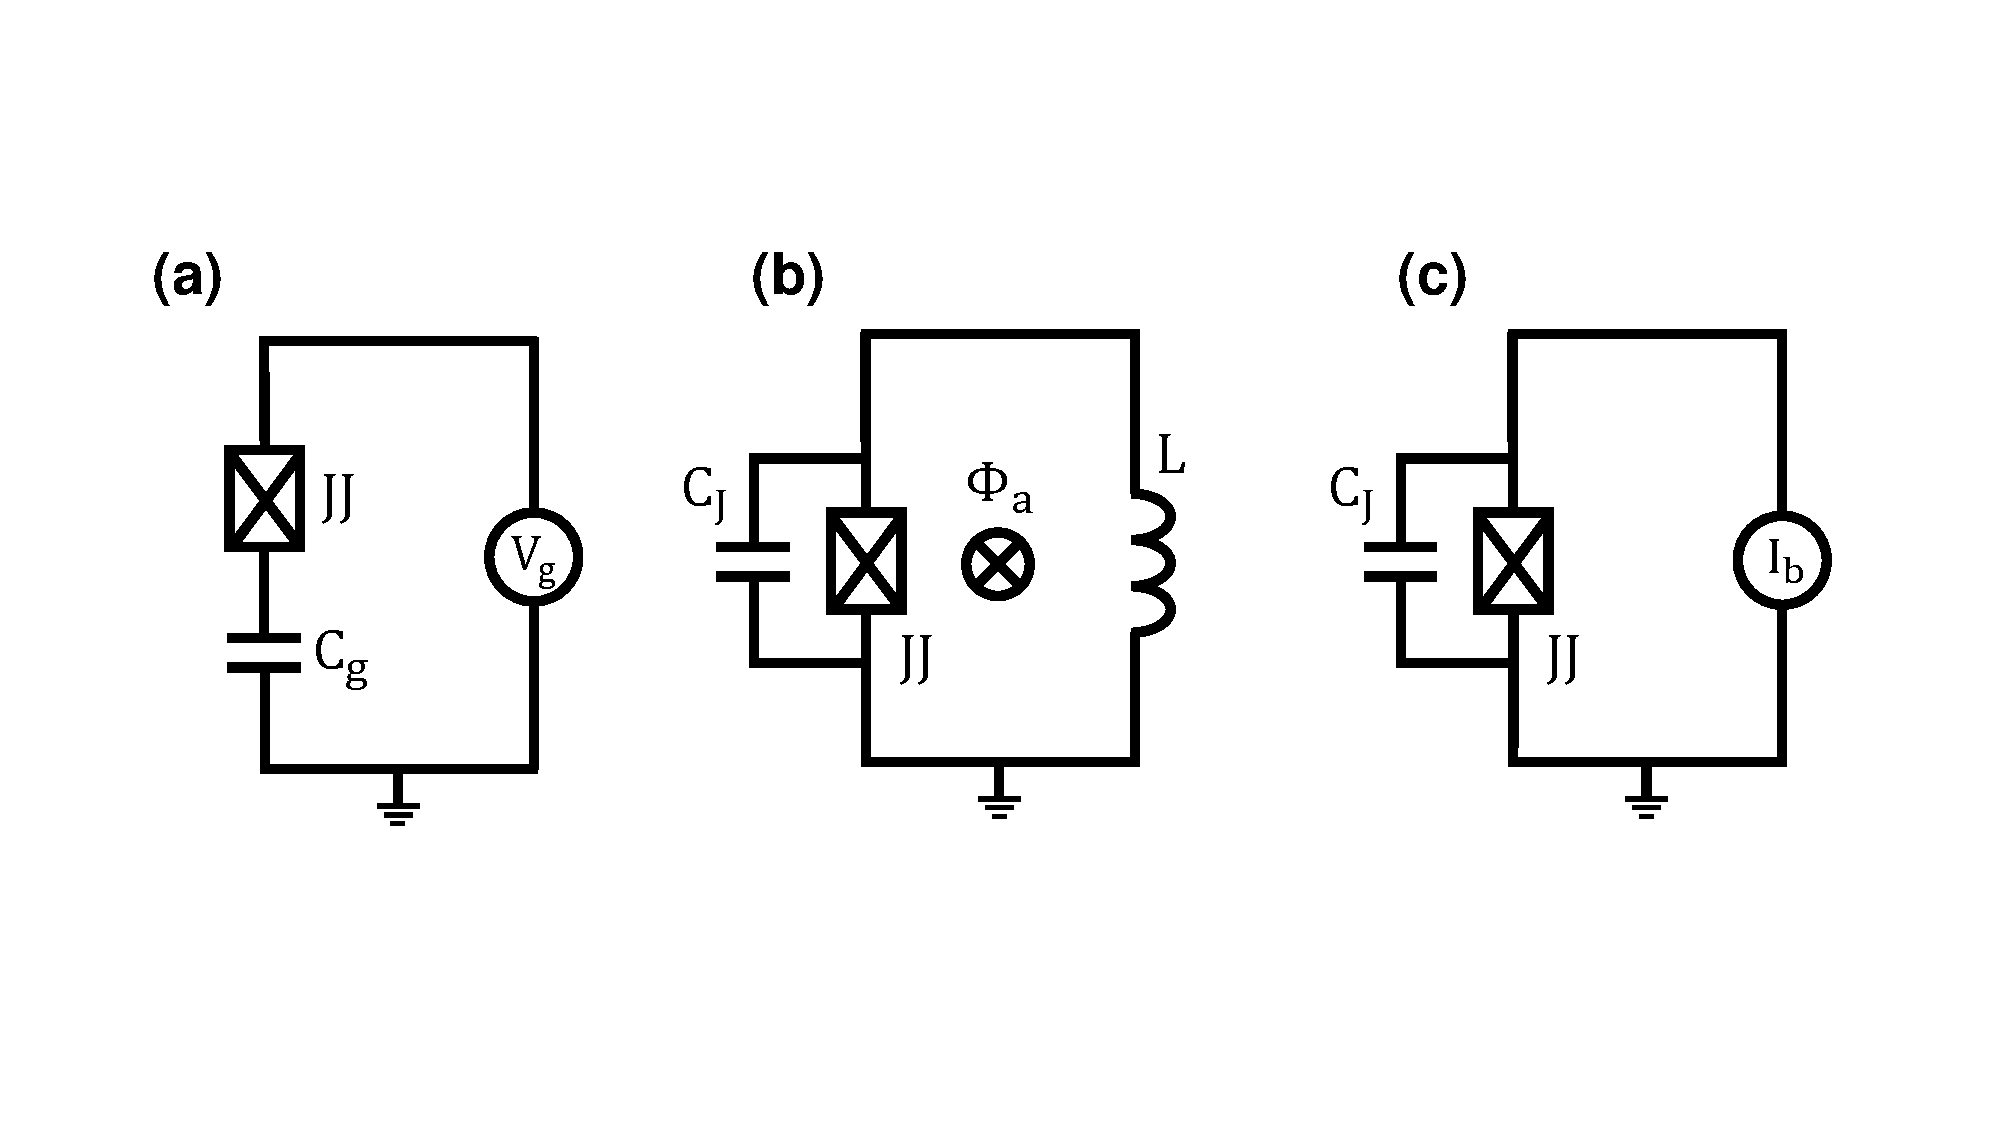
\includegraphics[width=0.9\textwidth]{ThreeQubit.pdf}
	\caption{电荷量子比特,磁通量子比特和相位量子比特电路示意图。(a)电荷量子比特:由一个约瑟夫森结和一个电容组成,调节偏置电压$ V_{g}$可以调节库伯对数目,进而调节比特频率。(b)磁通量子比特:由一个约瑟夫森结和一个环路电感组成,约瑟夫森结自身的电容充当比特电容,通过调节偏置磁通$ \Phi_{a}$调节比特频率。(c)相位量子比特:由约瑟夫森结和自身结电容组成比特,通过调节偏置电流调节比特频率。}
	\label{fig:ThreeQubit}
\end{figure}

为了减弱电荷噪声的影响,科研人员发明了一种新型的超导量子比特——传输子量子比特(transmon)\cite{koch2007charge},其示意图如图\ref{fig:transmon}a所示。传输子量子比特在电荷量子比特的基础上,在约瑟夫森结两端并联了一个大的电容,减小了$ E_{C}$,提高了$E_{J}/E_{C}$的比例。相应地,传输子量子比特对环境中的电荷噪声的敏感程度也将以$ {e}^{-\sqrt{8E_{J}/E_{C}}}$的关系式被指数级地抑制\cite{koch2007charge},现在传输子量子比特的寿命最高能达到$\rm 500 \ \mu s$\cite{wang2021transmon}。

\begin{figure}[h]
	\centering
	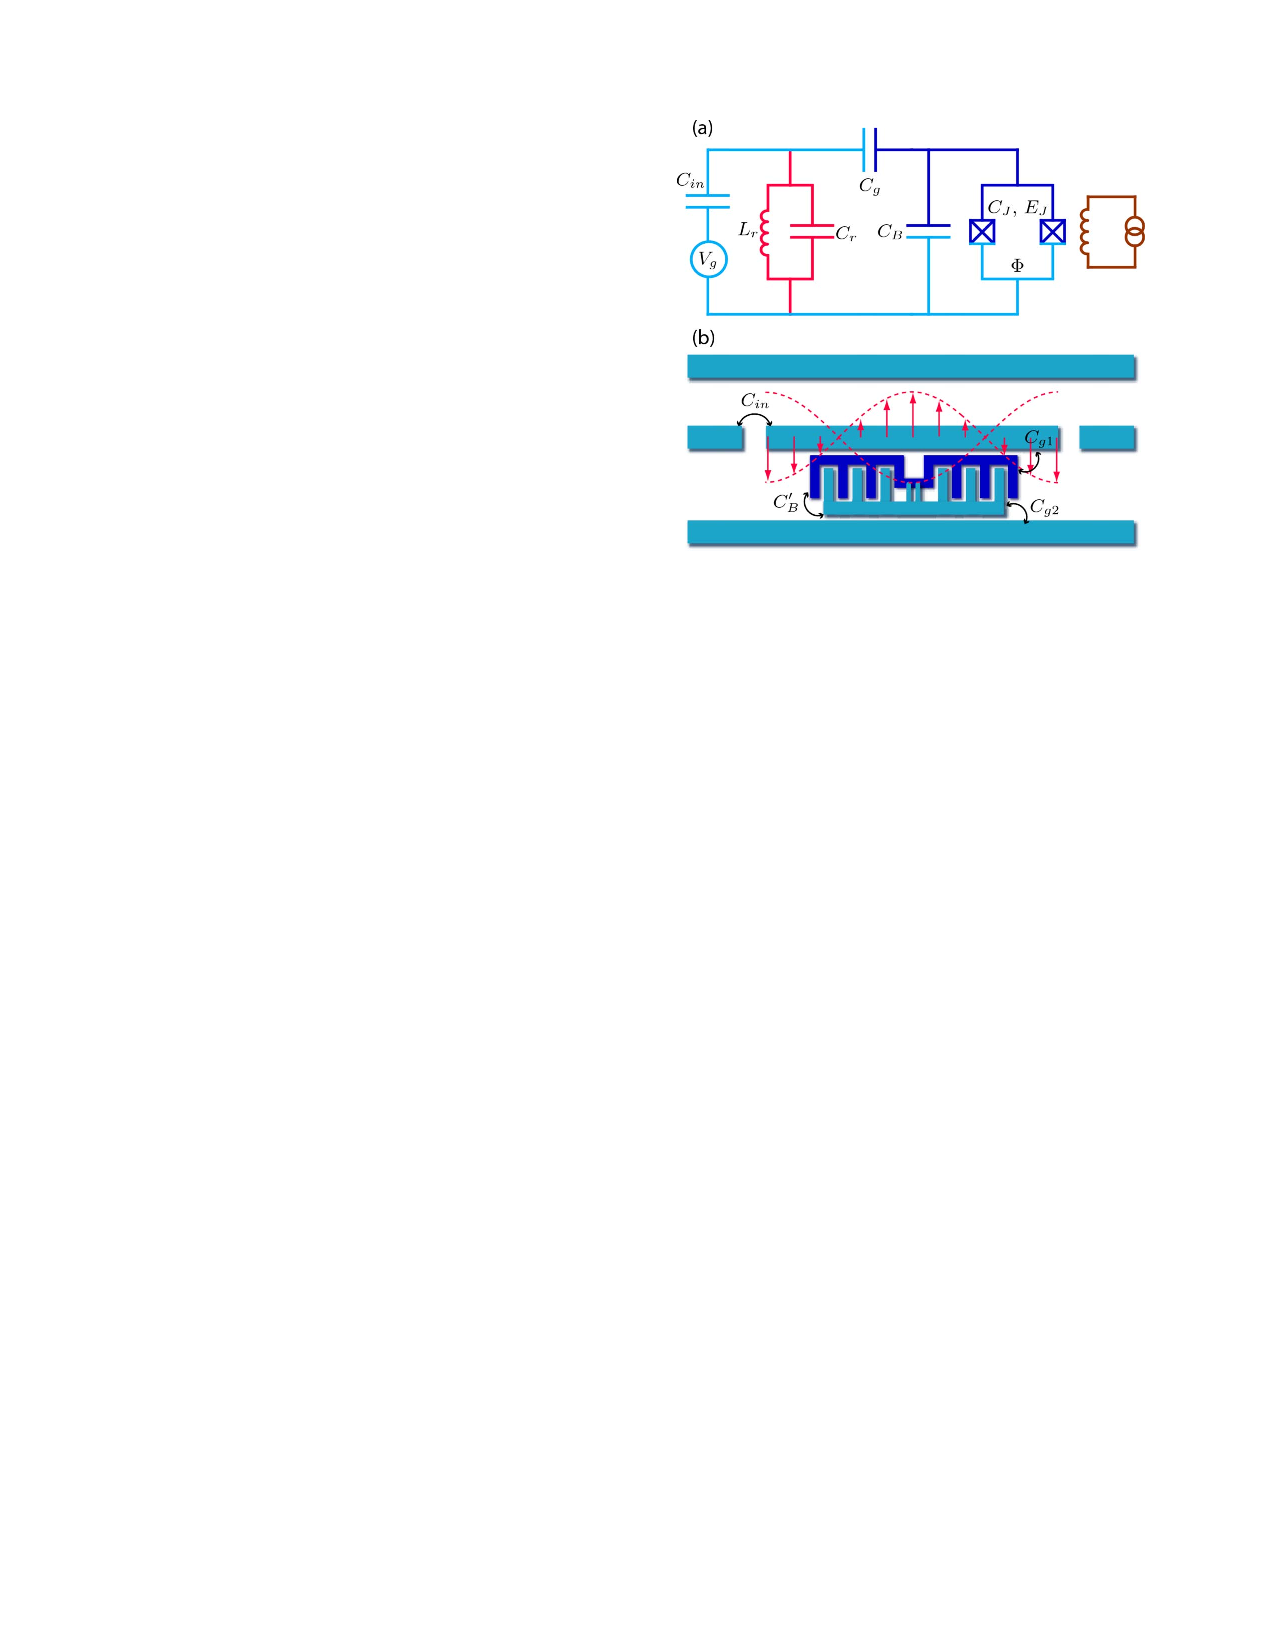
\includegraphics[width=0.8\textwidth]{transmon.pdf}
	\caption{传输子量子比特示意图\cite{koch2007charge}。(a)传输子量子比特的等效电路图。两个约瑟夫森结组成的dc-SUQID被一个大电容$ C_{B}$分流,以此减小充电能$ E_{C}$,提高了$ E_{J}/E_{C}$,减小了量子比特对电荷噪声的敏感程度。(b)传输子量子比特设计示意图。传输子量子比特内置在一个$ \dfrac{\lambda}{2}$传输线谐振腔内部,通过传输子量子比特与传输线谐振腔的耦合进行状态读取。}
	\label{fig:transmon}
\end{figure}

在此基础之上,去掉外接偏置电压源,并将约瑟夫森结另一端接地,构成接地传输子量子比特\cite{barends2013coherent}。接地传输子量子比特以其相干时间长、拓展性强,制备工艺简单的优点,已经成为应用最为广泛的超导量子比特之一。在我们的超导量子计算处理器中,主要采用的就是接地传输子量子比特,接下来介绍量子比特的基本性质就以接地传输子量子比特为例。

想要了解量子比特的基本性质,首先要了解接地传输子量子比特的电路结构及其对应的哈密顿量。
接地传输子量子比特电路结构如图所示\ref{fig:EL}b。根据其电路结构,我们可以观察到接地传输子量子比特是由一对并联约瑟夫森结和一个大电容并联接地所构成的。其哈密顿量可以写为:
\begin{equation}\label{XmonHamilton}
	\hat{H} =  4E_{C}\hat{n}^{2}-E_{J}\cos\left(\hat{\varphi}\right),
\end{equation}
其中$\hat{\varphi}$是dc-SQUID两端的相位差,$\hat{n}$是电容上存储的电荷对数目,$ \hat{\varphi}$和$ \hat{n}$满足对易关系$ [\hat{\varphi},\hat{n}]={i}$。$E_{C}$是表征电容存储能量的物理量,$ E_{J}=\dfrac{2I_{0}\Phi_{0}}{2\pi}\lvert \cos(\pi \dfrac{\Phi_{a}}{\Phi_{0}}) \rvert$为并联约瑟夫森结的总体约瑟夫森能,受到外界磁通$ \Phi_{a} $的调制,这也是超导量子比特频率可调的根源。

利用数值方法计算此哈密顿量的本征值,即可获得量子比特系统的能级结构,如图\ref{fig:EL}d所示。$\ket{1}$和$\ket{2}$能级之间的距离,明显不同于$\ket{0}$与$\ket{1}$能级之间的距离,这说明在约瑟夫森结的非线性作用下,$\ket{0}$与$\ket{1}$能级和其他能级分隔开,整个系统约化成一个二能级的量子比特系统。

在具体的量子比特设计中,$ E_{J}/E_{C}$的比例一般选择在$50\sim100$。在这个范围的设计参数下,接地传输子量子比特系统可以被看作一个小球在一个深度很深的余弦形的陷阱中运动,并且运动的速度相对较小。因此,粒子的运动范围主要局限在陷阱的最低点,即零点附近,$\varphi$的取值接近于0,小球所感受到的势能更接近于二次型的势能。以此为依据,我们可以将余弦势阱在零点附近进行泰勒展开,并截取势能的前三项$ 1-\varphi^{2}/2+\varphi^{4}/24$。泰勒展开后的系统哈密顿量可以近似写为:
\begin{equation}
	H = 4E_{C}\hat{n}^{2}-\dfrac{E_{J}}{2}\hat{\varphi}^{2}+\dfrac{E_{J}}{24}\hat{\varphi}^{4},
\end{equation}
此哈密顿量的前两项是LC谐振子哈密顿量,第三项就是引入的非线性势能项。非线性势能项也可以看作微扰项。对其进行二次量子化,得到系统的哈密顿量为:
\begin{equation}\label{XmonHamilton}
	H = \sqrt{8E_{J}E_{C}}\left( \hat{a}^{\dagger}\hat{a}+1/2 \right)-\frac{E_{C}}{12}\left( \hat{a}+\hat{a}^{\dagger}\right)^{4},
\end{equation}
第一项是谐振子哈密顿量,第二项是微扰项。微扰项为系统引入非简谐性。根据式\ref{XmonHamilton},利用微扰论的方法进行能级计算,可以近似得到能级$ \ket{j}$和能级$ \ket{j+1}$之间的能量差为:
\begin{equation}
	\hbar\omega_{j+1,j} = \sqrt{8E_{C}E_{J}}-E_{C}\left( j+1 \right),
\end{equation}
因此,量子比特$\ket{0}$、$ \ket{1}$能级间的能量差为$ \hbar\omega_{01} = \sqrt{8E_{C}E_{J}}-E_{C}$。定义量子比特的非简谐性$ \eta$为$ \ket{1}$、$\ket{2}$能级间的能量差和$\ket{0}$、$\ket{1}$能级间能量差的差值,即$\hbar\eta=\hbar\omega_{12}-\hbar\omega_{01}=-E_{C}$。

引入非简谐性后,$ \ket{0}$能级,$ \ket{1}$能级就与其他能级分隔开,形成一个由$ \ket{0}$和$\ket{1}$展开的计算子空间,这就构成了一个量子比特。在这个计算空间内,量子比特的哈密顿量可以用Pauli算符表示:$ H = \dfrac{-\hbar\omega}{2}\hat{\sigma}^{z}$。

在量子计算的过程中,非简谐性影响信息脱离计算空间的困难程度,对于量子比特的精确操控具有重要意义。非简谐性越大,操控过程中信息泄露出计算空间就越困难,量子比特操控的精度也就越高。但是增大非简谐性需要增大$ E_{C}$,这会同时以指数形式$ {e}^{-\sqrt{8E_{J}/E_{C}}}$增大量子比特对电荷噪声的敏感程度。所以要对两种影响做一个权衡,选择一个合适的$ E_{C}$、$ E_{J}$比例。最终,在我们的量子比特设计中,选择$ E_{C}=250 \  {MHz}$,$ E_{J}=14 \ {GHz}$,对应$ \ket{0}$能级、$ \ket{1}$能级频率差差$ \omega_{01}/2\pi=5 \ {GHz}$,非简谐性$ \eta/2\pi = -250\ {MHz}$。

\subsection{超导量子比特间的相互耦合}
对于一个量子计算过程,仅仅拥有相互独立的多个单独比特是不足够的,还需要多个量子比特间的相互作用,从而完成比特间信息的交换,构成任意的一个多比特演化矩阵,即完整的多量子比特计算过程。为了实现多比特间的相互作用,需要将两个量子比特相互耦合。比特间的耦合方式有许多种:电容直接耦合,电感直接耦合,谐振腔耦合,耦合器耦合等。电容直接耦合的方式是其中最为简单的,也是其他耦合方式的基础,所以下面主要介绍比特间的电容直接耦合。

比特间的电容直接耦合形式如下图\ref{fig:QQ}a所示。
以此可以得到系统的哈密顿量为:
\begin{equation}
		H= \frac{1}{2}{Q}^{T}{C^{-1}}{Q}-E_{J1}\cos(\varphi_1)-E_{J2}\cos(\varphi_2)
\end{equation} 
其中$Q$是电容上积累的电荷量,以矢量的形式表示,${C^{-1}}$是电容矩阵${C}$的逆矩阵,表此三者达式为:
\begin{align}
	{\Phi} &= \left(\begin{array}{l}
		\Phi_{1}\\
		\Phi_{2}
	\end{array}
	\right),\\
	{C} &= \left(\begin{array}{cc}
		C_{1}+C_{g} & -C_{g}\\
		-C_{g} & C_{2}+C_{g}
	\end{array}
	\right),	
\end{align}
\begin{equation}
	\begin{split}
		{C^{-1}} & =  \dfrac{1}{C_{1}C_{2}+C_{1}C_{g}+C_{2}C_{g}}
		\left(
		\begin{array}{cc}
			C_{2}+C_{g} & C_{g}\\
			C_{g} & C_{1}+C_{g}
		\end{array}
		\right) ,\\
		&=\left(
		\begin{array}{cc}
			C_{1}^{'-1} & C_{g}^{'-1}\\
			C_{g}^{'-1} & C_{2}^{'-1}
		\end{array}
		\right).
	\end{split}		
\end{equation}

\begin{figure}[h]
	\centering
	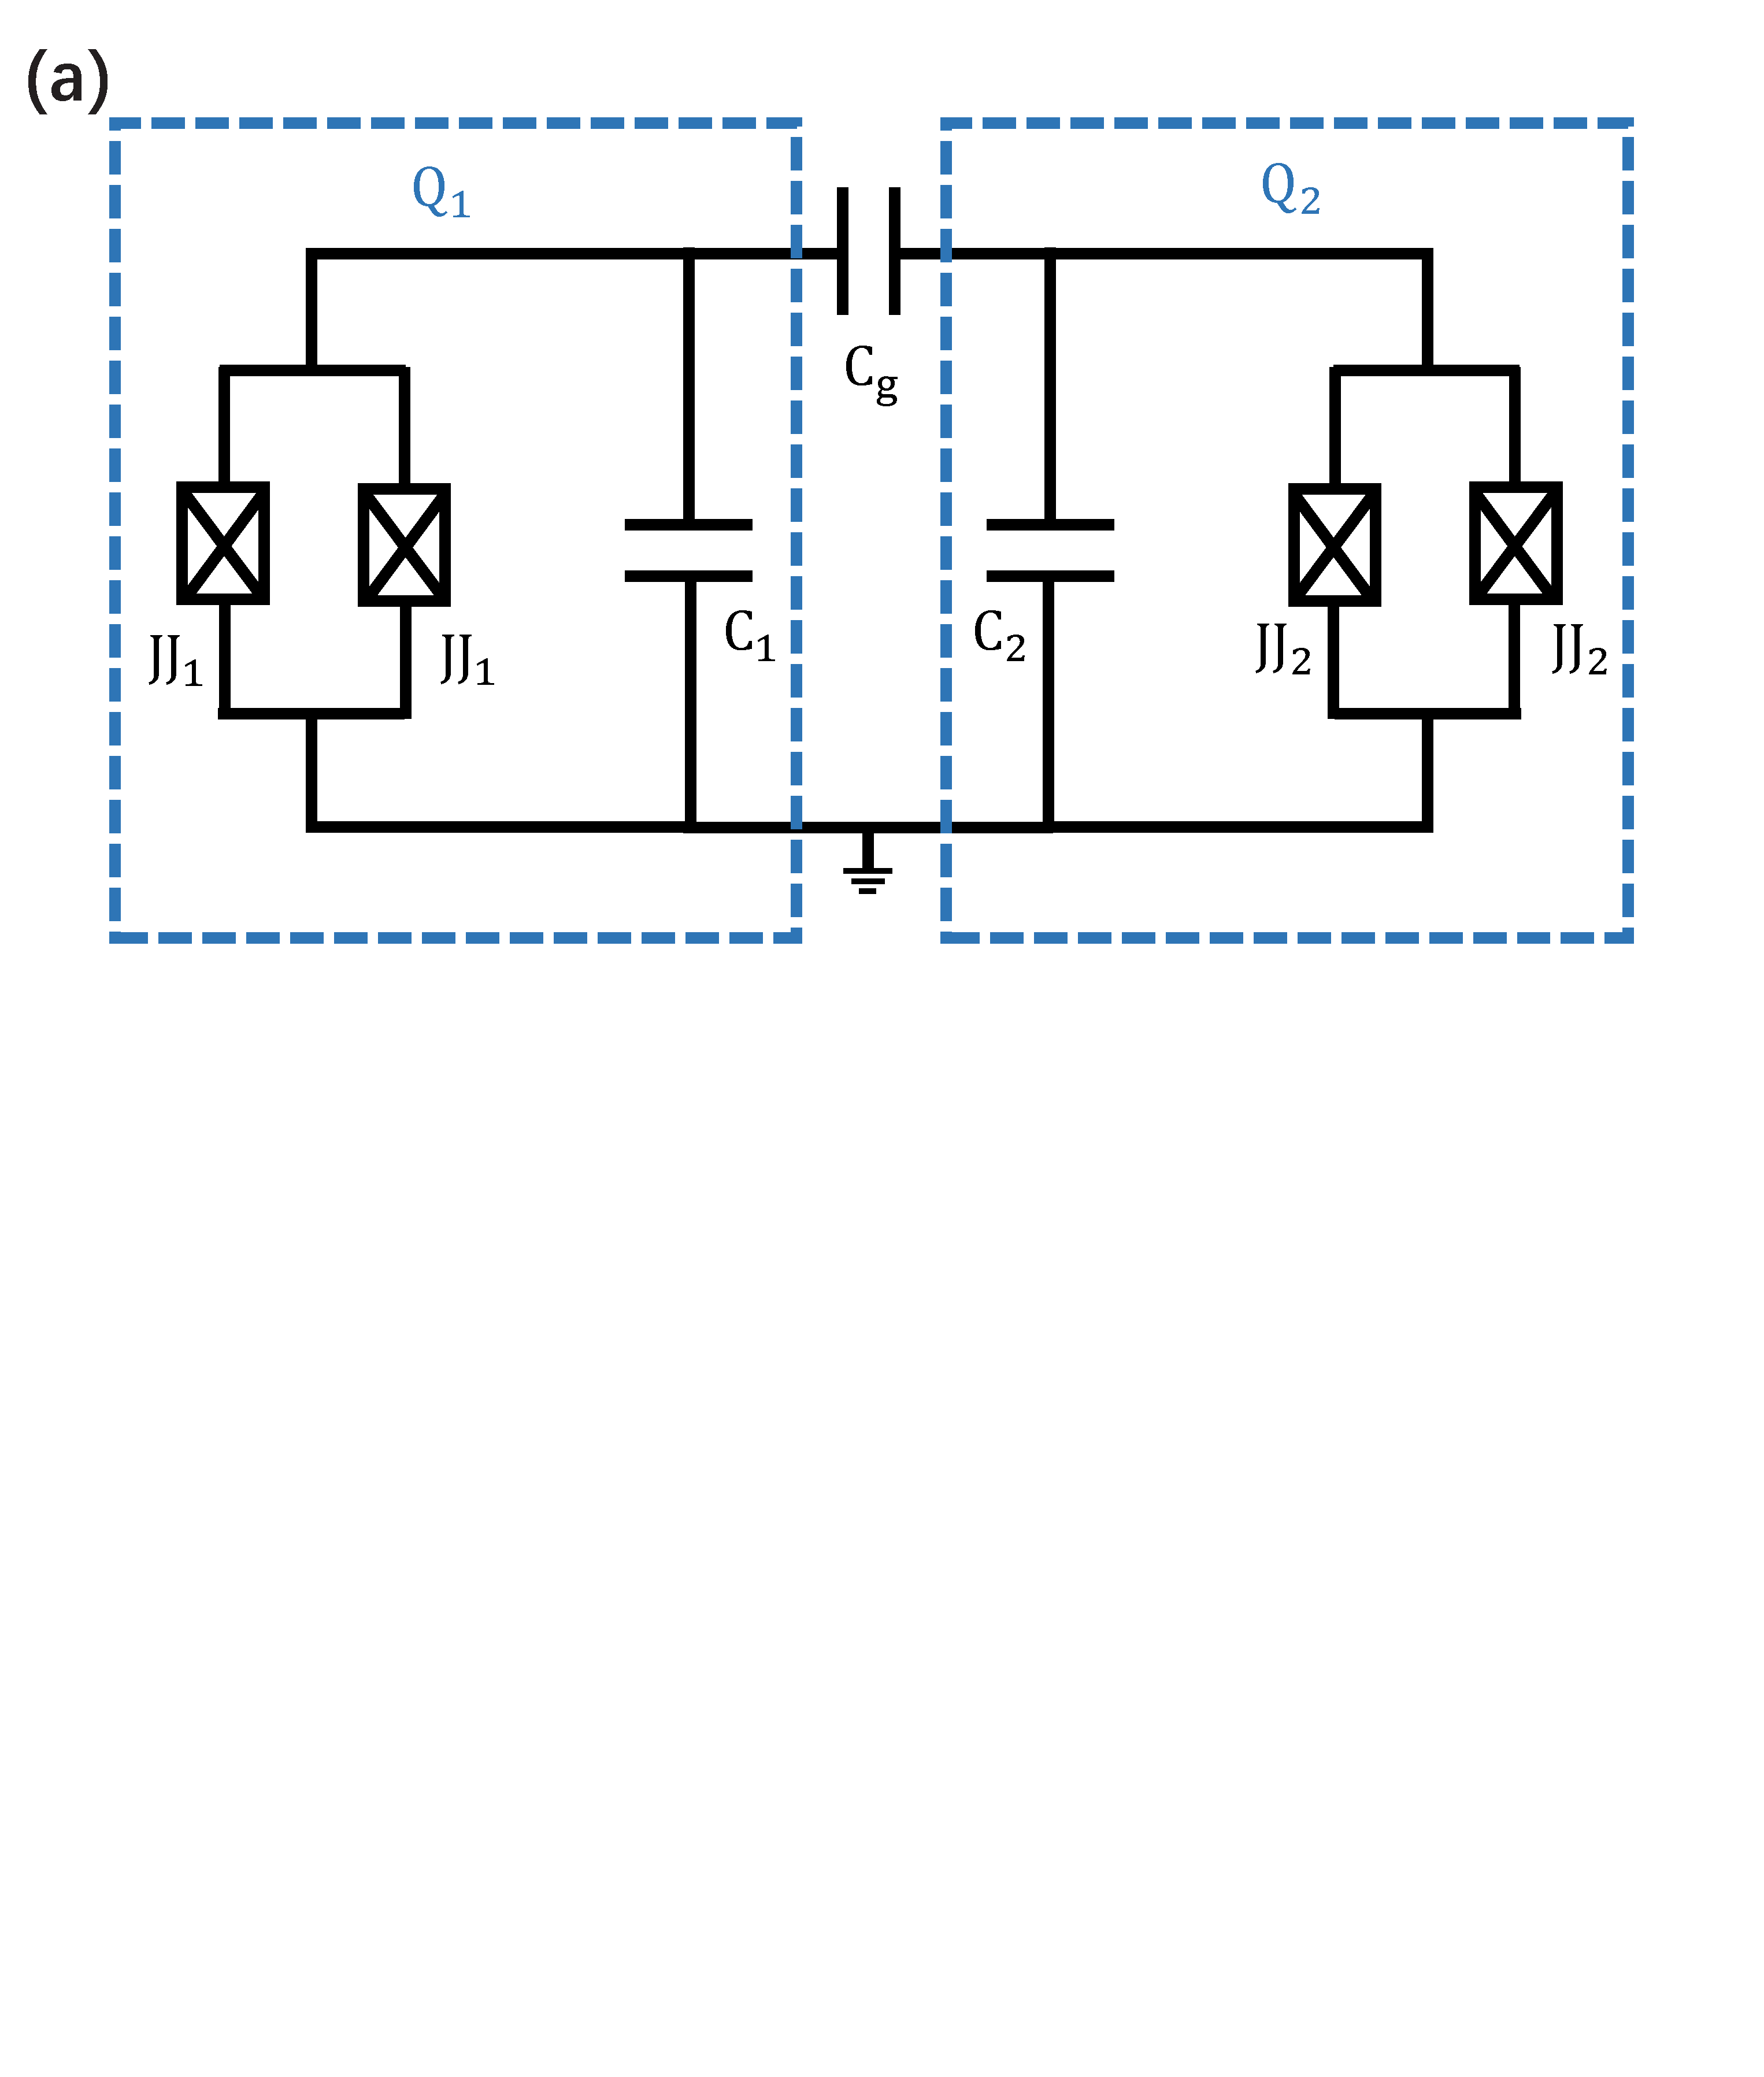
\includegraphics[width=0.9\textwidth]{QQ.pdf}
	\caption{量子比特间耦合系统电路示意图。两个量子比特$Q_{1}$和$Q_{2}$,通过耦合电容$C_{g}$进行耦合。}
	\label{fig:QQ}
\end{figure}

将矩阵形式的哈密顿量展开后,其表达式为:
\begin{equation}
	\begin{split}
		H &= \dfrac{Q_{1}^{2}}{2C_{1}^{'}} - E_{J1}\cos(\varphi_1)\\
		&+\dfrac{Q_{2}^{2}}{2C_{2}^{'}} - E_{J2}\cos(\varphi_2)\\
		&+\dfrac{Q_{1}Q_{2}}{C_{g}^{'}},
	\end{split}
\end{equation}
第一行和第二行的四项是两个比特的静态哈密顿量,第三行的第五项就是比特间的耦合哈密顿量。对此系统哈密顿量进行二次量子化,将整个系统转换到粒子数表象,并且只考虑二能级的计算空间,则系统的哈密顿可以表示为:
\begin{equation}
	H = -\dfrac{\hbar\omega_{1}}{2}\sigma^{z}_{1}-\dfrac{\hbar\omega_{2}}{2}\sigma^{z}_{2}+(\dfrac{E_{J1}E_{J2}}{4E_{C1}E_{C2}})^{1/4}\dfrac{{e}^{2}}{C_{g}^{'}}\sigma^{y}_{1}\sigma^{y}_{2},
\end{equation}
其中$E_{Ci}=\dfrac{{e}^2}{2C_{i}^{'}}$,是比特$i$的充电能量。前两项是两个比特各自的静态哈密顿量,比特$ i $的频率$ \hbar\omega_{i}=\sqrt{8E_{Ci}E_{Ji}}-E_{Ci}$。第三项是两个比特间的耦合项,耦合强度可以定义为:
\begin{equation}
	\begin{split}
		\hbar g &= (\dfrac{E_{J1}E_{J2}}{4E_{C1}E_{C2}})^{1/4}\dfrac{{e}^{2}}{C_{g}^{'}},\\
		&=\sqrt{\omega_{1}\omega_{2}}\dfrac{\sqrt{C_{1}^{'}C_{2}^{'}}}{2C_{g}^{'}}.
	\end{split}
\end{equation}

简化后的哈密顿量可以表示为:
\begin{equation}
	H/\hbar = -\dfrac{\omega_{1}}{2}\sigma^{z}_{1}-\dfrac{\omega_{2}}{2}\sigma^{z}_{2}+g\sigma^{y}_{1}\sigma^{y}_{2},
\end{equation}

在耦合项$g\sigma^{y}_{1}\sigma^{y}_{2}$的作用下,两个比特间的信息可以相互交换。利用这种方式,我们可以构成量子线路中的双比特门,从而构成一个完整的量子计算过程。双比特门的具体构成方式,会在后面介绍。
\subsection{其他形式的超导量子比特}
在本节中,我们将简要介绍除了transmon外,其余几种比较常用的超导量子比特。
\subsubsection{Three-junction flux qubit}
three-junction flux qubit是Mooij在1999年提出的,由包含三个约瑟夫森结的小环路构成,如图\ref{fig:3-JJ}所示。量子比特的$\ket{0}$态和$\ket{1}$态分别由环路中的顺时针电流和逆时针电流所编码,且可以调节控制线中的电流信号,改变感应磁通,进而控制比特状态。通过减小环路的大小,还可以有效量子比特对磁通噪声的敏感程度。
\begin{figure}[h]
	\centering
	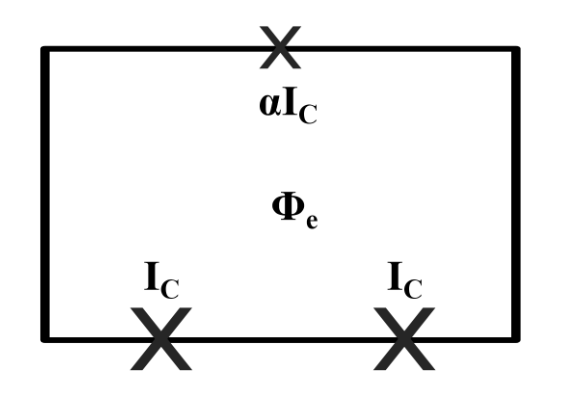
\includegraphics[width=0.6\textwidth]{3-JJ.png}
	\caption{Three-junction flux qubit的电路结构示意图。两个约瑟夫森结具有相同的约瑟夫森能量$E_{J}$,第三个约瑟夫森结具有更小的约瑟夫森能量$\alpha E_{J}$}
	\label{fig:3-JJ}
\end{figure}
\subsubsection{C-shunt flux qubit }
C-shunt flux qubit是You在2007年所提出的,是对three-junction flux qubit的改进。在three-junction flux qubit中,磁通噪声被有效抑制,电荷噪声成为主要噪声源,因此在约瑟夫森结两端并联一个大电容,可以有效减小系统的充电能,降低系统对电荷噪声的敏感程度,提高量子比特的相干时间。具体结构如图\ref{fig:Cshunt}所示。
\begin{figure}[h]
	\centering
	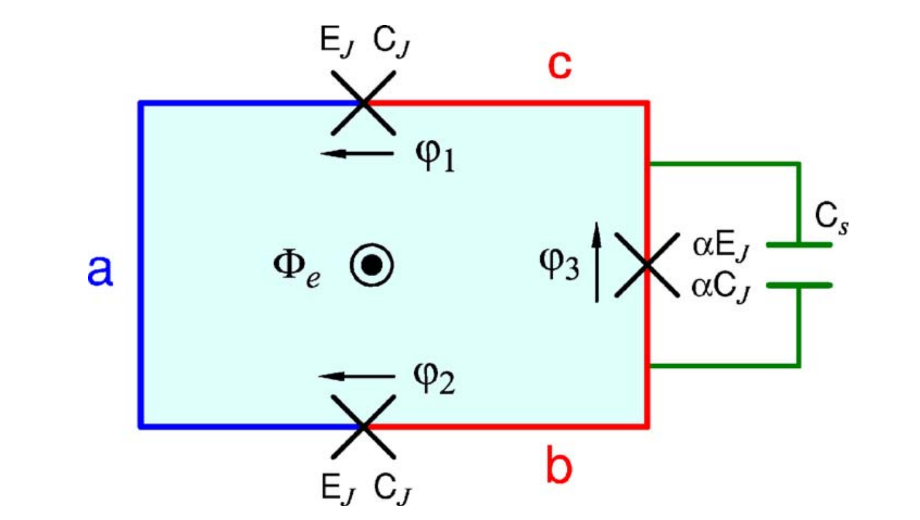
\includegraphics[width=0.6\textwidth]{Cshunt.png}
	\caption{C-shunt flux qubit的电路结构示意图。结构与three-junction flux qubit的电路结构类似,只是电容$C_{s}$并联在小的约瑟夫森结旁。}
	\label{fig:Cshunt}
\end{figure}
\subsubsection{Fluxonium}
Fluxonium是Manucharyan在2009年提出的,目的是降低低频电荷噪声的影响。Fluxonium的电路结构如图\ref{fig:Fluxonium}所示,是一系列串联的大电容约瑟夫森结和一个小电容约瑟夫森结所构成。在比特工作频率,一系列串联的约瑟夫森结可以被看作一个接地大电感,相当于一个低通滤波器。通过这种方式,低频电路噪声被短路接地了,量子比特对低频电荷噪声的的敏感程度也被降低了,其相干时间最高能提高到$1 ms$。
\begin{figure}[h]
	\centering
	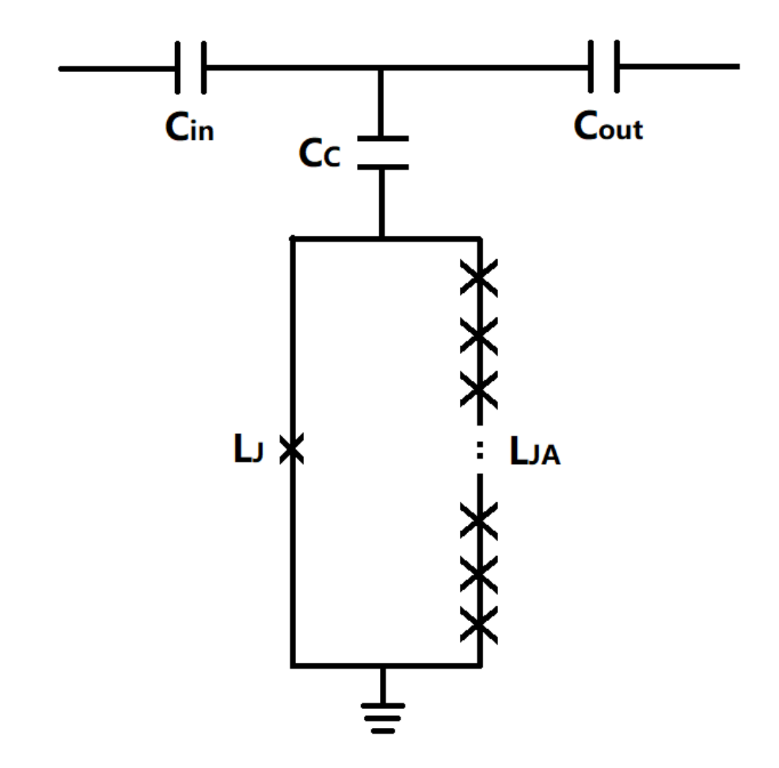
\includegraphics[width=0.6\textwidth]{Fluxonium.png}
	\caption{Fluxonium的电路结构示意图}
	\label{fig:Fluxonium}
\end{figure}

\subsubsection{$0-\pi$ qubit}
$0-\pi$ qubit由Kitaev, Brooks 和 Preskill提出,并于2019年被Gyenis实验实现。其电路结构如下图\ref{fig:0-pi}A所示。此电路结构构成了一个双势阱系统,其势能结构如下图\ref{fig:0-pi}B所示。两个势阱的底部分别对应系统的$\ket{0}$态和$\ket{1}$态。两个势阱之间的势垒比较高,因此$\ket{0}$态和$\ket{1}$态之间的传输矩阵元也比较小,对磁通噪声和电荷噪声都不敏感,具有很强的相干性能。

\begin{figure}[h]
	\centering
	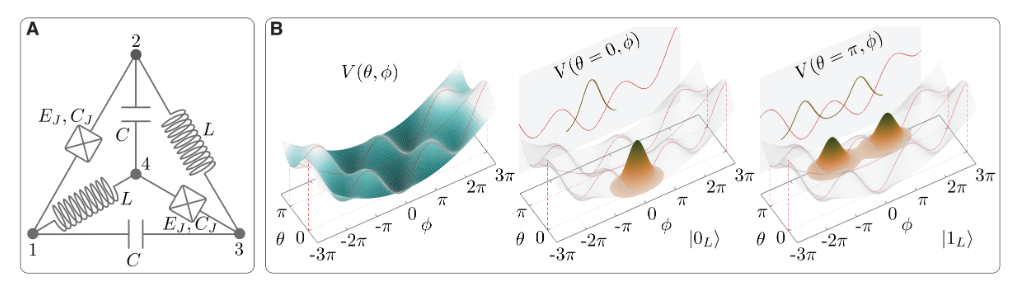
\includegraphics[width=0.9\textwidth]{0-pi.png}
	\caption{$0-\pi$ qubit的结构示意图。A)$0-\pi$ qubit的电路结构示意图。B)$0-\pi$ qubit的势能结构示意图。}
	\label{fig:0-pi}
\end{figure}
\section{测量与控制系统}
测量与控制系统是整个超导量子计算系统正常运行的关键,其包含两部分:
第一部分是稀释制冷机系统,其为超导量子计算处理器提供了一个低噪声的运行环境,避免了量子比特受到热,磁通等噪声的干扰\cite{bertet2005dephasing,kumar2016origin};第二部分是测控信号产生与传输系统,它根据具体的实验需求,在室温端生成所需的测控信号,通过低温传输线路系统和微波封装系统将测控信号传输到量子比特上,操控量子比特完成特定的演化过程。
\subsection{稀释制冷机系统}
在对超导量子计算处理器进行测量与控制时,需要为量子计算处理器维持一个极低温的环境,其主要原因有两点:第一点是金属铝膜需要进入超导状态。量子比特的核心部件是约瑟夫森结,只有铝金属膜进入超导状态,形成超导约瑟夫森结,才能让量子比特呈现正常的比特功能。此外,铝金属膜进入超导状态,也会有效减小量子比特的损耗,增大比特的退相干时间。第二点是热噪声对量子比特有显著影响。热噪声会影响比特的$\ket{1}$态激发与能量弛豫,设计的超导量子比特常见频率$ f_{01}$为$\rm 5 \ GHz$,对应的特征温度$ T_{Q} = hf_{01}/k_{b}=240\ {mK}$。为了让周围环境的热噪声对量子比特的影响可以忽略,需要使得周围环境温度$T_{env}$满足,量子比特稳态热激发数$P_{Thermal}=e^{-T_{Q}/T_{env}}\ll 1$的条件。

因此,在考虑维持的低温温度时,需要同时对这两方面进行考虑。
超导量子比特中常用的铝,铌,铟金属的超导转变温度$T_{c}$分别为$\rm 1.18 \ K$,$\rm 9.25 \ K$,$\rm 3.41 \ K$,因此需要将环境温度降至转变温度$ T_{c}$以下。此外,环境温度$ T_{env}$还需要满足$ P_{Thermal}=e^{-T_{Q}/T_{env}}\ll 1 $的条件。综上考虑以上两点因素后,比特周围的环境温度至少要降低到$\rm 100 \ mK$以下,所以设计使用稀释制冷机系统对超导量子计算处理器进行冷却。稀释制冷机系统的构造如下图\ref{fig:BlueForsStructure}所示,从上到下有五层法兰盘,分别是$\rm 50 \ K$层,$\rm 4 \ K$层,still层,cold plate层和Mixing chamber层。超导量子计算处理器就被安装在Mixing Chamber层,该层的裸机温度能降低到$\rm 10 \ mK$以下。

\begin{figure}[h]
	\centering
	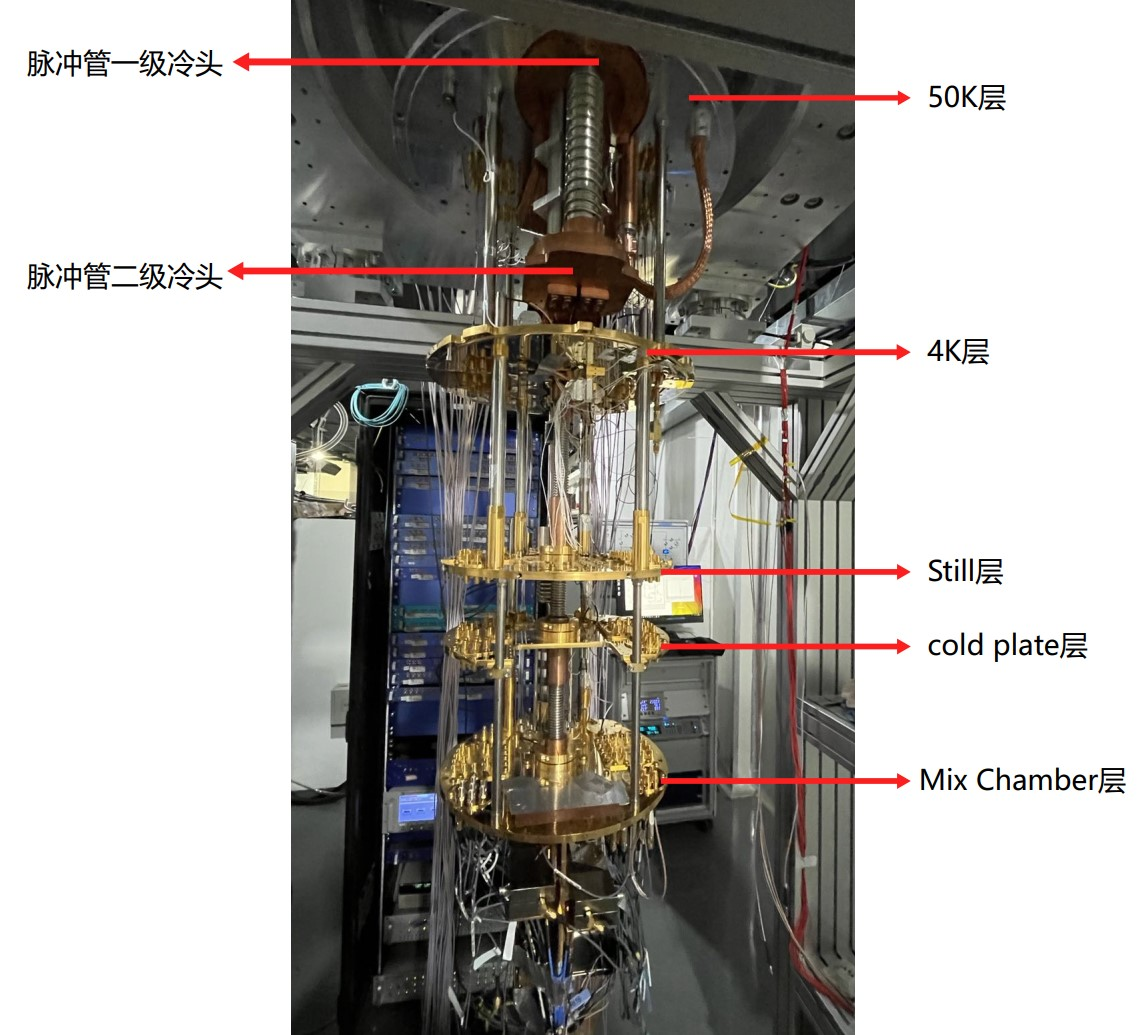
\includegraphics[width=0.8\textwidth]{BlueForsStructure.jpg}
	\caption{稀释制冷机结构示意图。}
	\label{fig:BlueForsStructure}
\end{figure}
\subsection{控制与测量信号的产生与传输系统}
超导量子比特需要被外界施加信号才能进行特定动力学演化与比特状态测量。所以需要在室温产生控制与测量信号,并将其通过低温传输线路系统和微波封装系统传输到量子比特上,进而实现量子比特的控制与测量。
\subsubsection{室温信号发生与采集系统}
室温信号发生与采集系统由任意波发生器(AWG),微波源,直流源,室温放大器,时钟系统,数据采集系统(DAQ)等器件组成,具体结构如下图\ref{fig:electrics}所示。

\begin{figure}[h]
	\centering
	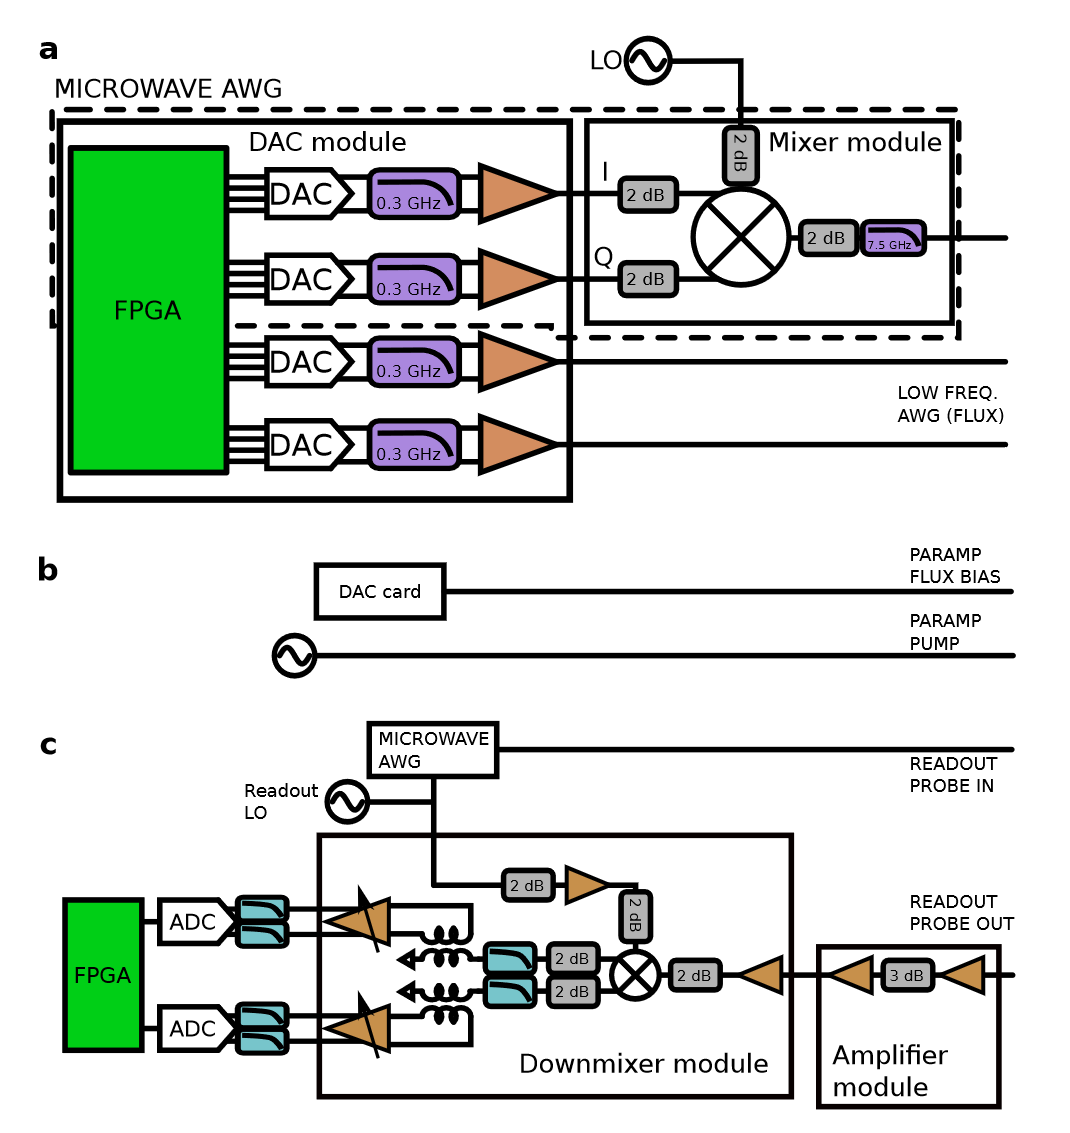
\includegraphics[width=0.6\textwidth]{electrics.png}
	\caption{室温信号发生与采集系统示意图。a)XY控制信号和快Z控制信号的室温发生系统。b)控制放大器的XY控制信号和慢Z信号的室温发生系统。c)读取信号的室温发生与采集系统。}
	\label{fig:electrics}
\end{figure}


对于量子比特的控制,需要产生两种控制信号:一种是XY控制信号,用以控制量子比特的状态;另一种是Z控制信号,用以控制量子比特的频率,Z控制信号分为慢Z信号和快Z信号,慢Z信号将量子比特长时间稳定地偏置到idle频率;快Z信号将量子比特从idle频率快速偏置到工作频率。

关于XY控制信号的产生,我们使用AWG产生频率在$\rm 500 MHz$以内的微波信号,再和微波源信号经过混频器上转换得到频率在$\rm 5 GHz$左右的微波信号,以此作为XY控制信号。关于Z控制信号的产生,我们使用AWG产生脉冲信号作为快Z信号,使用直流源产生偏置电流作为慢Z信号,二者在制冷机内通过加法器合成最终的偏置Z信号。

对于量子比特的读取,系统中只有一种读取信号。读取信号的产生与XY控制信号类似,AWG产生的微波信号和微波源信号经过混频器上转换得到最终的读取信号。读取信号被输入到读取线路中,与量子比特的读取腔发生相互作用。量子比特的状态信息包含在从制冷机输出的读取信号的幅度与相位信息中。输出的读取信号经过室温放大器放大后,被数据采集系统所采集,经过下转换,模数转换,数字解调,得到读取信号在IQ平面上的位置,即是量子比特的状态信息。

时钟系统产生其他所有器件所需的时钟信号,保证所有设备同步有序工作。
\subsubsection{低温传输线路系统}
在室温产生量子比特的控制与测量信号后,测控信号需要通过低温传输线路系统在制冷机内部传播,最终传输到量子比特,与量子比特发生相互作用,完成量子比特状态的控制与读取。低温传输线路系统的具体结构如下图\ref{fig:LTWire}所示,包含同轴线,衰减器,滤波器,加法器,循环器,放大器等微波器件。

\begin{figure}[h]
	\centering
	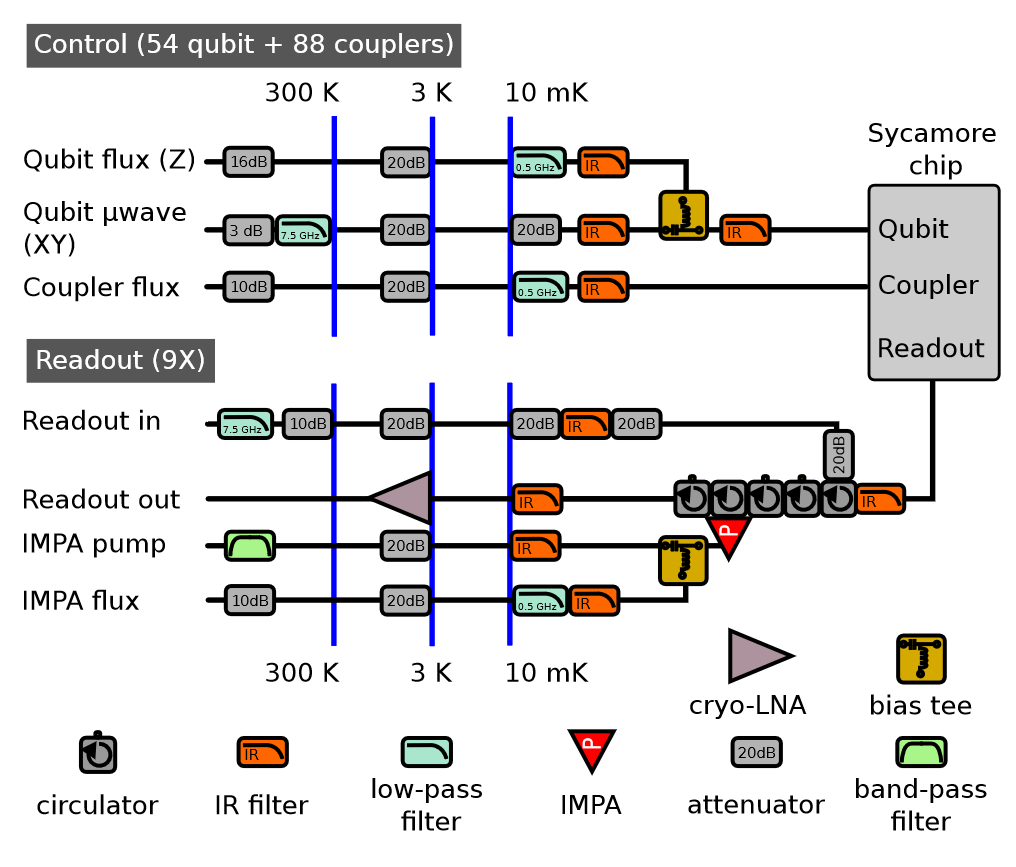
\includegraphics[width=0.9\textwidth]{LTWire.png}
	\caption{低温传输线路系统示意图。低温传输线路系统包含同轴线,衰减器,滤波器,加法器,循环器,放大器等微波器件,分别用于信号的传递,噪声的降低,以及信号的放大。}
	\label{fig:LTWire}
\end{figure}

衰减器和滤波器也是低温传输线路中广泛使用的微波器件。衰减器一般安装在各层法兰盘之上,主要有两个作用:一是衰减信号的强度。因为量子比特所需的信号强度很微弱,例如XY控制信号的电流强度仅是微安量级,如果在室温直接产生如此微弱的信号,室温热噪声的存在就会大大降低信号的信噪比。为了增大信噪比,在室温生成较强的信号,保证了比较高的信噪比,然后根据各级法兰盘的温度梯度,安装合适的衰减器,使得上一层的热噪声经过衰减后,与下一层的热噪声相当,以此保证通过测控信号经过衰减器逐级衰减,不会显著降低信噪比\cite{krinner2019engineering}。通过这种方式,量子比特获得了一个高信噪比的测控信号,可以以此完成精确的操控和读取;二是作为传输线的热沉,吸收电阻发热额外产生的热噪声,将每层传输线温度降低到对应层法兰盘的温度,避免额外热噪声的引入。


滤波器的主要功能是滤除不相关频段的噪声。对于XY控制信号和读取信号,主要应用信号频段为$\rm 4-8 \ GHz$;对于快Z控制信号,主要应用频段在$\rm 500 \ MHz$以内;对于慢Z信号,主要应用频段为接近直流的频段。因此,需要在低温传输线路中安装合适频段的滤波器,将不相关的频率滤除。对于读取信号线路和XY信号线路,会在Mixing Chamber层安装$\rm 8\ GHz$的低通滤波器,滤除$\rm 8\ GHz$以上的噪声;对于快Z信号线路,会在Mixing Chamber层先安装$\rm 500 \ MHz$的低通滤波器,再安装$\rm 8\ GHz$的低通滤波器。这是为了防止$\rm 500 \ MHz$的低通滤波器对于高频噪声的抑制效果不佳,所以增加一个$\rm 8\ GHz$的低通滤波器滤除高频噪声;与之类似的,会在慢Z信号线路的4K层安装RC滤波器,将$\rm KHz$级别以上的信号噪声滤除,又为了防止Still层热噪声的干扰,会在Mixing Chamber层先安装$\rm 80 \ MHz$的低通滤波器和$\rm 8\ GHz$的低通滤波器。这些滤波器都是为了滤除传输线路中更高频率的噪声,对于防止其对量子比特的干扰\cite{martinis2014ucsb}。

\section{总结}
在这一部分内容中,我们介绍了超导量子计算系统的结构,其主要分为超导量子处理器和信号产生与传输系统两部分。对于超导量子处理器,我们以传输子量子比特为例,详细介绍如何利用约瑟夫森结在能级等间隔的谐振子系统中引入非线性,将超导电路的多能级系统约化成超导量子比特的二能级,并且介绍如何利用电容将多个量子比特耦合起来,形成比特间的信息交换。此外,我们也介绍了其余几种常见的量子比特。

对于信号产生与传输系统,我们首先介绍稀释制冷机系统,这是维持处理器量子状态的基础。然后介绍了室温信号产生与采集系统以及低温传输线路系统,这部分系统帮助我们能够在室温通过经典电子学器件控制低温下超导量子比特的状态,进而完成量子计算过程。


